\chapter{\protect\textsc{Carico}}
% This chapter may be called something else\ldots but in general the
% idea is that you have one (or a few) ``meat'' chapters which describe
% the work you did in technical detail.
% \begin{tcolorbox}[boxsep=0mm,left=2.5mm,right=2.5mm]
    % \textbf{Design and Implementation:} {\em In this section, I will outline the
    % goals of my system. I will give a brief overview of the chapter structure,
    % summarising each core section and what I achieve.}
% \end{tcolorbox}
This chapter details \textsc{Carico}, a novel federated, asynchronous,
memory-limited algorithm, building upon the principles of \textsc{Pronto}.
Rather than performing standard FPCA, \textsc{Carico} applies FSVD on
non-centered metrics to build a model of experience resource usage. By combining
this model with a new continuous signal function, nodes can be scored by their
capacity according to the expected workload and their current resource usage.
Finally, we explain the two assumptions required to translate the calculated
capacity signal into one that can be reserved. As this algorithm produces a
signal that measures "capacity", I will refer to it as \textsc{Carico} - "load"
in Italian.

\section{Capacity Signal}
In Section \ref{sec:intro-weakness}, we identified critical limitations of
\textsc{Pronto}'s binary ``Reject-Job" signal within the Kubernetes ecosystem:
its lack of comparable Node scoring and inability to handle Pod startup
latencies. While one could conceivably compare the number of detected spikes,
this does not translate into a reservabl signal, meaning its imporssoble to
quantitavely assign or reserve ``peak detections" for incoming Pods.
Furthermore, as emprically demonstrated in Figure
\ref{fig:podcount-util-pressure}, contention metrics often do no change
proportionally to the number of tasks assigned, making them difficult to reserve
accurately.

To overcome these limitations, a signal reflecting varying levels of contention
and offering a predictable, scalar relationship with task assignments was
necessary. This led us to reconsider a metric of capacity. Supported by its use
within \texttt{kube-scheduler}, this approach provides the necessary properties
to make it suitable with reservation mechanisms. The subsequent challenge was to
adapt \textsc{Pronto}'s underlying mathematical framework, FSVD, to produce a
measure of capacity instead of performance variability. The goal was to develop
a continuous, comparable, and reservable signal that could effectively and
accurately guide scheduling decisions.

\section{Local Model}
\label{sec:local-model-construction}
In \textsc{Pronto}, iterative-SVD is performed on the mean-centered batch of CPU-Ready
samples and its latest local model. Iterative-SVD allows \textsc{Pronto} to become a
stream algorithm with memory usage proportional to $O(d)$ where $d$ is the
number of features in the batch. The resulting $U$ and $\Sigma$ matrix
correspond to the PCs of the latest data combined with historical data.

In \textsc{Carico}, the nodes perform iterative-SVD on a batch of [0,1]-normalised
telemetry data. The telemetry data must have the following property: a value of
0 indicates empty while a value of 1 indicates capacity is full. As we are
no-longer mean-centering the dataset before applying SVD, the value we are
maximising is:
\begin{align}
x_i^T \mathbf{A}^T \mathbf{A} x_i &= \left\| \begin{bmatrix}
\text{---} & x_i^T & \text{---} \\
\end{bmatrix}
\begin{bmatrix}
| \\
a_1 \\
|
\end{bmatrix} \quad \cdots \quad
\begin{bmatrix}
| \\
a_n \\
|
\end{bmatrix} \right\|^2 \\
&= \left( \begin{bmatrix}
\text{---} & x_i^T & \text{---} \\
\end{bmatrix}
\begin{bmatrix}
| \\
a_1 \\
|
\end{bmatrix} \right)^2 + \left( \begin{bmatrix}
\text{---} & x_i^T & \text{---} \\
\end{bmatrix}
\begin{bmatrix}
| \\
a_2 \\
|
\end{bmatrix} \right)^2 + \dots + \left( \begin{bmatrix}
\text{---} & x_i^T & \text{---} \\
\end{bmatrix}
\begin{bmatrix}
| \\
a_n \\
|
\end{bmatrix} \right)^2
\end{align}

The $j^{\text{th}}$ term in the above equation is maximised by choosing $x_i =
a_j / ||a_j||$. Hence the $x_i$ that maximises the entire sum can bet
interpreted as a 'weighted average' over all $a_j$s. An $a_j$ with a greater
length representing higher resource usage will contribute more to the direction
of the unit vector $x_i$.

\section{Subspace Merging}
\label{sec:local-merge}
Given a new batch of samples $A'$, performing incremental-SVD to merge to get
the new PCA. As every element in $A$ and $A'$ is [0,1] normalised, the maximised
expression follows this property:
\begin{align}
x_i^T \mathbf{[AA']}^T \mathbf{[AA']} x_i &= \left\| \begin{bmatrix}
\text{---} & x_i^T & \text{---} \\
\end{bmatrix}
\begin{bmatrix}
| \\
a_1 \\
|
\end{bmatrix} \quad \cdots \quad
\begin{bmatrix}
| \\
a_{2n} \\
|
\end{bmatrix} \right\|^2 \\
&= \left( \begin{bmatrix}
\text{---} & x_i^T & \text{---} \\
\end{bmatrix}
\begin{bmatrix}
| \\
a_1 \\
|
\end{bmatrix} \right)^2 +  \dots + \left( \begin{bmatrix}
\text{---} & x_i^T & \text{---} \\
\end{bmatrix}
\begin{bmatrix}
| \\
a_{2n} \\
|
\end{bmatrix} \right)^2 \\
&\geq \left( \begin{bmatrix}
\text{---} & x_i^T & \text{---} \\
\end{bmatrix}
\begin{bmatrix}
| \\
a_1 \\
|
\end{bmatrix} \right)^2 + \dots + \left( \begin{bmatrix}
\text{---} & x_i^T & \text{---} \\
\end{bmatrix}
\begin{bmatrix}
| \\
a_{n} \\
|
\end{bmatrix} \right)^2
\end{align}

As $\sigma_i$ corresponds to $\text{Var}_i$, with each iterative-SVD, we
increase the eigenvalues of $\Sigma$. This is problematic as exploding values
can result in more expensive matrix operations. In addition, both \textsc{Pronto} and
\textsc{Carico} use $\Sigma$ as some sort of weighting. Unreasonably large $\sigma_i$
values will result in incorrect signal values.
\begin{align}
    & \textbf{B} = \left[\bigg(\frac{\sqrt{\alpha}}{\sqrt{\alpha +
    \beta}}\mathbf{A}\bigg)\bigg(\frac{\sqrt{\beta}}{\sqrt{\alpha +
    \beta}}\mathbf{A'}\bigg)\right] \\
& x_i^T \mathbf{B}^T\mathbf{B} x_i = \frac{\alpha}{\alpha + \beta}\left\| \begin{bmatrix}
\text{---} & x_i^T & \text{---} \\
\end{bmatrix}
\begin{bmatrix}
| \\
a_1 \\
|
\end{bmatrix} \quad \cdots \quad
\begin{bmatrix}
| \\
a_{n} \\
|
\end{bmatrix} \right\|^2 + \\
& \hspace{2.2cm} \frac{\beta}{\alpha + \beta}\left\| \begin{bmatrix}
\text{---} & x_i^T & \text{---} \\
\end{bmatrix}
\begin{bmatrix}
| \\
a_{n+1} \\
|
\end{bmatrix} \quad \cdots \quad
\begin{bmatrix}
| \\
a_{2n} \\
|
\end{bmatrix} \right\|^2\\
    &\therefore \min(\text{Var}_i(\textbf{A}), \text{Var}_i(\textbf{A}')) \leq
    \text{Var}_i(\textbf{B}) \leq \max(\text{Var}_i(\textbf{A}),
    \text{Var}_i(\textbf{A}'))
\end{align}
However, scaling the concatenated matrix using the method above can upper
and lower bound the growth of $\Sigma$. This also effectively behaves as an EMA,
as each contribution of the previous sample is reduced by $\alpha / (\alpha +
\beta)$.

\section{Capacity Signal}
\label{sec:capacity-signal}
From the model section, we understood $\textbf{U}$ as the orthonormal vectors
that maximise the projected squared distance of the telemetry dataset
$\mathbf{A}$. As every element in $\mathbf{A}$ is in the range [0,1], $u_1$
within $\mathbf{U}$ will have either all positive or all negative values. This
means that the other orthonormal vectors $u_2, \ldots, u_n$ will have at least
one element that differs in sign from another. As a result, the remaining
eigenvalues of $\mathbf{U}$ are not valide resource-usage directions: $\forall 1
< i < n, k \neq 0: \exists j \in {1,\ldots,n} \text{ such that} (ku_i)_j \le 0$.
As a result, only $u_1$ gives us a meaningful result: a weighted average of
resource usage.

From this we can build a new capacity signal that considers both the estimated
workload resource usage and its current resource usage. Given the current
workload $y$, $u_1$ and $\sigma_1$ from the latest $U$ and $\Sigma$, a Node's
estimated capacity signal $k$ is given by:
\begin{align}
    y_{\text{predict}} = y + k * \sqrt{\sigma_1} u_1 \\
    \max_k \forall i: y_{\text{predict}} < 1
\end{align}

As $\sigma_1$ is the sum of the projected square distances of the recent
workload, we can scale $u_1$ by this distance to represent the size of expected
workload. We could have also averaged the squared distance using
$\sqrt{\sigma_1/b}$, but this would just scale $k$ for all nodes and not
provide any more information.

\subsection{Example Scenarios}
\label{sec:signal-example-scenario}
To better understand how this signal works, I will explore how the signal
changes under different different loads. This scenarios will also be used to
control the correctness of the signal implementation in the prototype.

\begin{figure}[H]
    \centering
    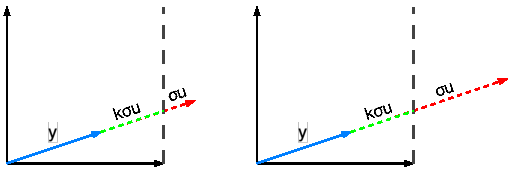
\includegraphics[width=\textwidth]{images/conflicting-workload.pdf}
    \caption{Visualisations of a Node's resource usage $y$ and expected resource
    usage $\sigma_1 u_1$ when learning of conflicting resource utilisation.}
    \label{fig:conflicting-workload}
\end{figure}

Figure \ref{fig:conflicting-workload} presents the scenario where a Node updates
its local model, learning that the experienced workload has increased in
resource usage ($\sigma_1$ has increased). This means that a smaller constant
$k$ is needed before the combined vectors cross a resource boundary. As a
result, a Node advertises a smaller capacity signal as it has less capacity for
the expected resource usage.

\begin{figure}[H]
    \centering
    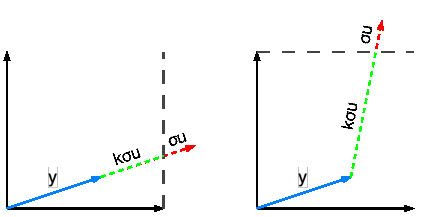
\includegraphics[width=0.8\textwidth]{images/complementary-workload.pdf}
    \caption{Visualisations of a Node's resource usage $y$ and expected resource
    usage $\sigma_1 u_1$ when learning of complementary resource utilisation.}
    \label{fig:complementary-workload}
\end{figure}

Figure \ref{fig:complementary-workload} presents the scenario where a Node updates
its local model, learning that the learned workload is using more resources but
in a different direction. This could be described as a complementary workload as
the the dot product of the current resource utilisation and the expected
resource utilisation is much smaller. Therefore, a larger constant $k$ is needed
to cross a resource boundary. This results in a Node advertising a higher
capacity signal as it has more capacity for the new expected resource
utilisation.

\section{Reserve Cost and Capacity}
\label{sec:spazio-cost-capacity}
Like \textsc{Pronto}, \textsc{Carico}'s signal uses its current resource usage, and therefore, only
reflects Pods that have been scheduled and are running on the Node. For \textsc{Carico}
to work in a system with Pod startup latency, the scheduler must be able to
predict the effect a Pod will have on a Node's signal. \textsc{Carico} assumes that Nodes
know the number of currently running Pods, as well as, have the ability to
estimate their signal capacity and per-Pod cost (I will explain the prediction
methods used in the prototype in section \ref{}). From With information, a Node
can calculate its available capacity from:
\begin{align}
    \text{avail.} &= \frac{\text{signal}}{\text{per-Pod cost}} \\
    \text{avail.} &= \frac{\text{capacity}}{\text{per-Pod cost}} - \text{pod
    count}\\
\end{align}
This metric has two useful properties:
\begin{itemize}
    \item \textbf{Dual-Mode:} The available capacity can be calculated
        using two equations. This is especially useful in Kubernetes as during
        the creation or deletion of a Pod, the current measured resource usage
        can experience large spikes. To combat this noise, Nodes can switch to
        predicting available capacity using estimated capacity and Pod count.
        This reduces fluctuations in a Node's advertised capacity and improves
        scheduling decisions
    \item \textbf{Unit of Measure:} This metrics' unit of measure is Pod count.
        Sending the latest signal, capacity and per-pod-cost values would
        increase the amount of data sent between Nodes and increase the
        complexity of the central scheduler's algorithm.
\end{itemize}

Each Node $n$ will broadcast its $\text{avail.}_n$ to a central scheduler. This
scheduler also tracks each Node's reserved amount as $\text{reserved}_n$. For
each Pod waiting to be assigned to a Node, the scheduler performs the following
operations:
\begin{itemize}
    \item \textbf{Filter:} Filters out all Nodes $n$ with $\text{avail.}_n -
        \text{reserved}_n < 1$. Ensures we do not schedule on Nodes that do not
        have enough resources for another pod.
    \item \textbf{Score:} Score Nodes $n$ by $\text{avail.}_n -
        \text{reserved}_n$. This ensures we allocate to Nodes which can fit more
        Pods.
    \item \textbf{Reserve:} Once a node is Node has been chosen, we increment
        $\text{reserved}_n$ by $1$ for that Node. Once a scheduled Pod is no
        no longer in the Pending state, the central scheduler decrements
        $\text{reserved}_n$ by $1$ for the Node $n$ the Pod was assigned to.
\end{itemize}

\section{Properties}
\textsc{Pronto} is designed to be \textit{federated, streaming} and
\textit{unsupervised}. \textsc{Carico} exhibits identical properties while also
considering the existance of communication and Pod startup latency.

\textbf{Federated:} \textsc{Pronto} executes scheduling plans in a decentralised fashion
without knowledge of the global performance dataset. Such approach in
Kubernetes could actually decrease performance. The Kubernetes API server
handles the publishing and updating of Kubernetes objects. A decentralised
system with no global synchronisation or coordination could result in a
stampede of Bind requests that could overload the Kubernetes API server and slow
down the publishing of incoming Pods. Instead, \textsc{Carico} uses a central scheduler
to score Nodes and perform the final Bind operation. However, it can still be
considered federated because of its use of federated PCA \cite{}: individual
Nodes can have a unified view of the global workload while maintaining their
individual autonomy to set their score as they deem fit.

\textbf{Streaming:} \textsc{Carico}'s use of iterative-SVD, like \textsc{Pronto}, means it only
requires memory linear to the number of features considered; the required memory
is proportional to $\mathcal{O}(d)$. Furthermore, like \textsc{Pronto}, \textsc{Carico} only
requires a single pass over the incoming data without having to store historical
data in order to update its estimates.

\textbf{Unsupervised:} \textsc{Carico} uses a derivative of PCA, a popular technique for
discovering linera structure or reducing dimensionality in data. Like \textsc{Pronto}, it
exploits the resulting subspace estimate along with the incoming data to reveal
patterns in recent resource-usage.

\textbf{Continuous Value} \textsc{Pronto} is a binary signal, which makes difficult to
score Nodes. \textsc{Carico}'s $\text{avail.} \in \mathbb{R}$, allowing Nodes to be
filtered and scored against each other.

\textbf{Latency Resilient:} Unlike \textsc{Pronto} which assumes no communication
latency, \textsc{Carico} was designed with Kubernetes in mind, and thus must consider
possible latency in communication and Pod startup. \textsc{Carico}'s $\text{avail.}$'s
unit of measure allows the central scheduler to easily track the estimated cost
of Pods in-flight, ensuring subsequent scheduling decisions do not mistakenly
overload a Node with a high $\text{avail.}$.
%
% There are several methods to integrating the reserve cost into the signal to be
% sent to the central scheduler. The first method involves sending the signal and
% the reserve cost as separate values. On pod bind, we reserve the latest pod cost
% from the signal, and only relinquish the reserved amount once the central
% scheduler \verb|kube-apiserver| listener detects the pod is no longer Pending.
% This method requires the central scheduler to keep track of both the pods on
% each node and the pod-cost when the pod was bound.
%
% I instead chose to integrate the reserve quantity directly into the signal: each
% node calculates its available capacity in terms of no. of pods using two equations:
% \[ \text{avail. capacity from signal} = \frac{\text{signal}}{\text{per-pod-cost}} \\
   % \text{avail. capacity from no. of pods} = \frac{\text{capacity}}{\text{per-pod-cost}} -
   % \text{no. of pods} \]
%
% We use to functions for different situations. Typically, we calculate the
% available capacity from the latest signal measurements. However, if we detect a
% recent container event, the remote \verb|pronto| pod calculates the capacity
% from the pod count. This is to reduce the instability introduced by the
% container runtime. Furthermore, with this signal, the central scheduler does not
% have to record the per-pod-cost at bind time as the signal is now given in terms
% of individual pod counts. This simplifies the central scheduler and reduces the
% memory demand on.
%
